\chapter{Methodology}
\label{chap:methodology}

This chapter describes the proposed system. It begins with the workflow of the current manual process and the automated workflow that replaces part of it, then presents the architecture of the three functional groups, the algorithm of each module, the training configuration and the implementation details.

The system comprises six main functions:

\begin{itemize}
    \item \textbf{Box/Envelope Detection:} determines whether the postal item is a parcel or an envelope.
    \item \textbf{Information Region Detection:} locates the region containing information on the parcel surface.
    \item \textbf{Handwriting Recognition:} detects text regions, recognizes the handwriting and converts the output into structured data.
    \item \textbf{Dimension Measurement Using Computer Vision:} measures parcel dimensions with two webcams, YOLO and image processing.
    \item \textbf{Dimension Measurement Using Ultrasonic Sensors:} measures dimensions with three ultrasonic sensors and an ESP32.
    \item \textbf{Shipping Fee Calculation:} normalizes province and city names, determines the route, computes the chargeable weight and calculates the shipping fee.
\end{itemize}

\section{Business Process Analysis}
\label{sec:bpa}

The current manual workflow at the acceptance counter is illustrated in Figure~\ref{fig:currentprocess}: read the information, enter the data, weigh the item, read the weight, enter the weight, measure the dimensions, enter the dimensions, determine the chargeable weight, select the service, calculate the fee, check and confirm.

\begin{figure}[htbp]
\centering
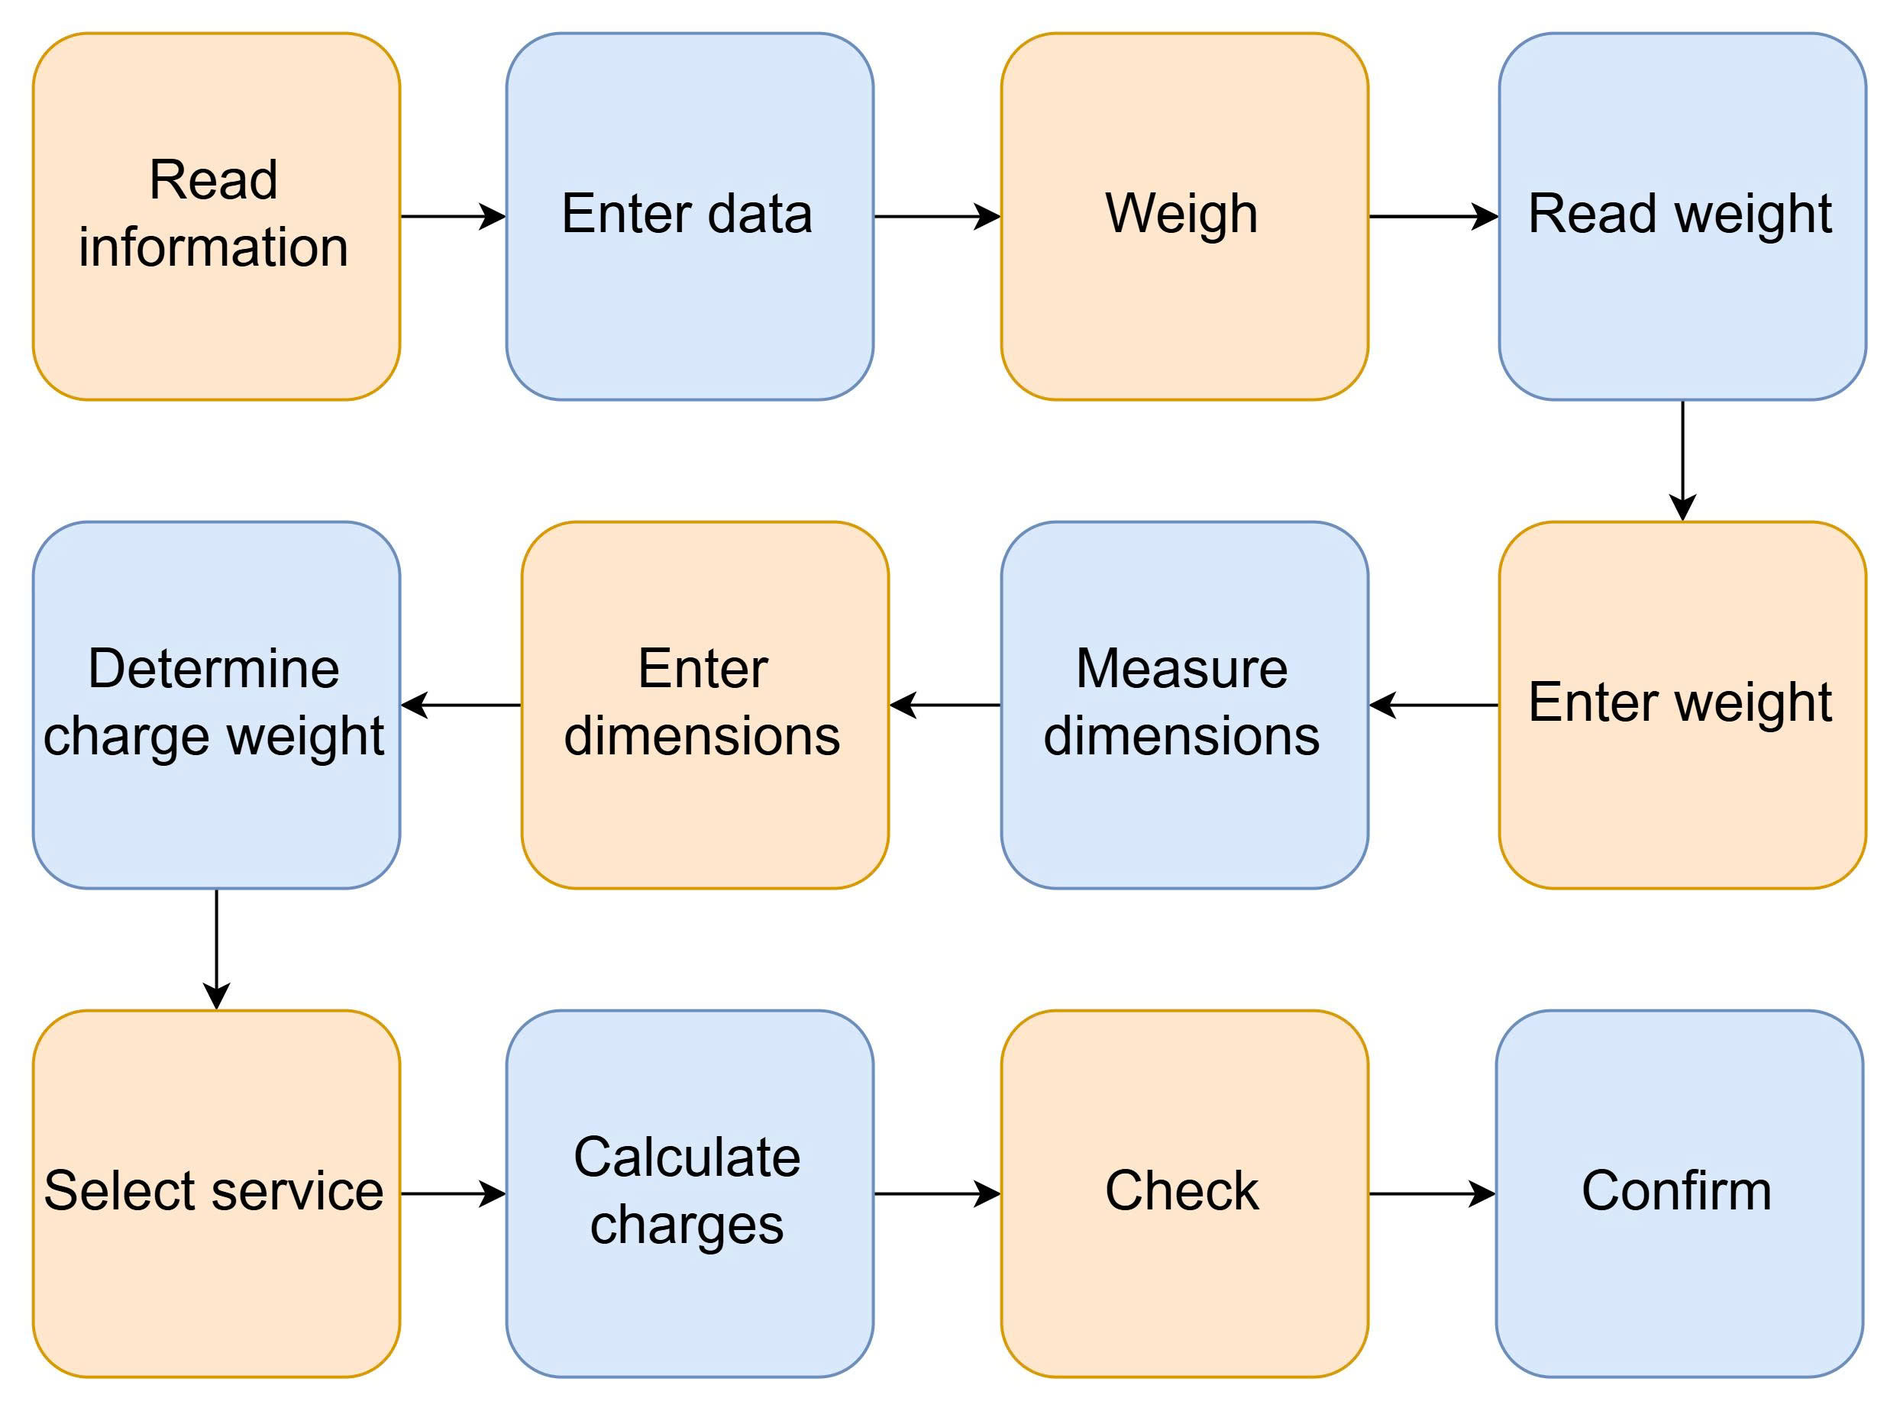
\includegraphics[width=0.92\textwidth]{Images/fig4_1.png}
\caption{Current postal item handling process at the acceptance counter.}
\label{fig:currentprocess}
\end{figure}

In practice, completing a typical postal transaction currently takes about 6--8 minutes per item. Within that time the clerk must carry out many consecutive steps: receiving the request; reading or asking for sender and receiver information; entering names, phone numbers and addresses; checking the contents; weighing the item; measuring dimensions where required; entering the parameters into the software; determining the chargeable weight; selecting the service; determining the base fee, surcharges and value-added services; re-checking the information; printing the label or shipping form; collecting payment and completing the transaction. This description is based on the team's own observation of the acceptance counter.

The proposed system automates three groups of these steps. Reading information and entering data are replaced by automatic extraction of the information on the postal item using a handwriting OCR model. Measuring and entering dimensions are replaced by automatic parcel dimension measurement using USB webcams or ultrasonic sensors. Determining the chargeable weight, selecting the service and calculating the fee are replaced by automatic computation of the volumetric weight, service type determination and fee calculation.

\section{Overall Workflow}

Figure~\ref{fig:workflow} presents the processing flow of the proposed system, from receiving the input image to saving the result in the database.

\begin{figure}[htbp]
\centering
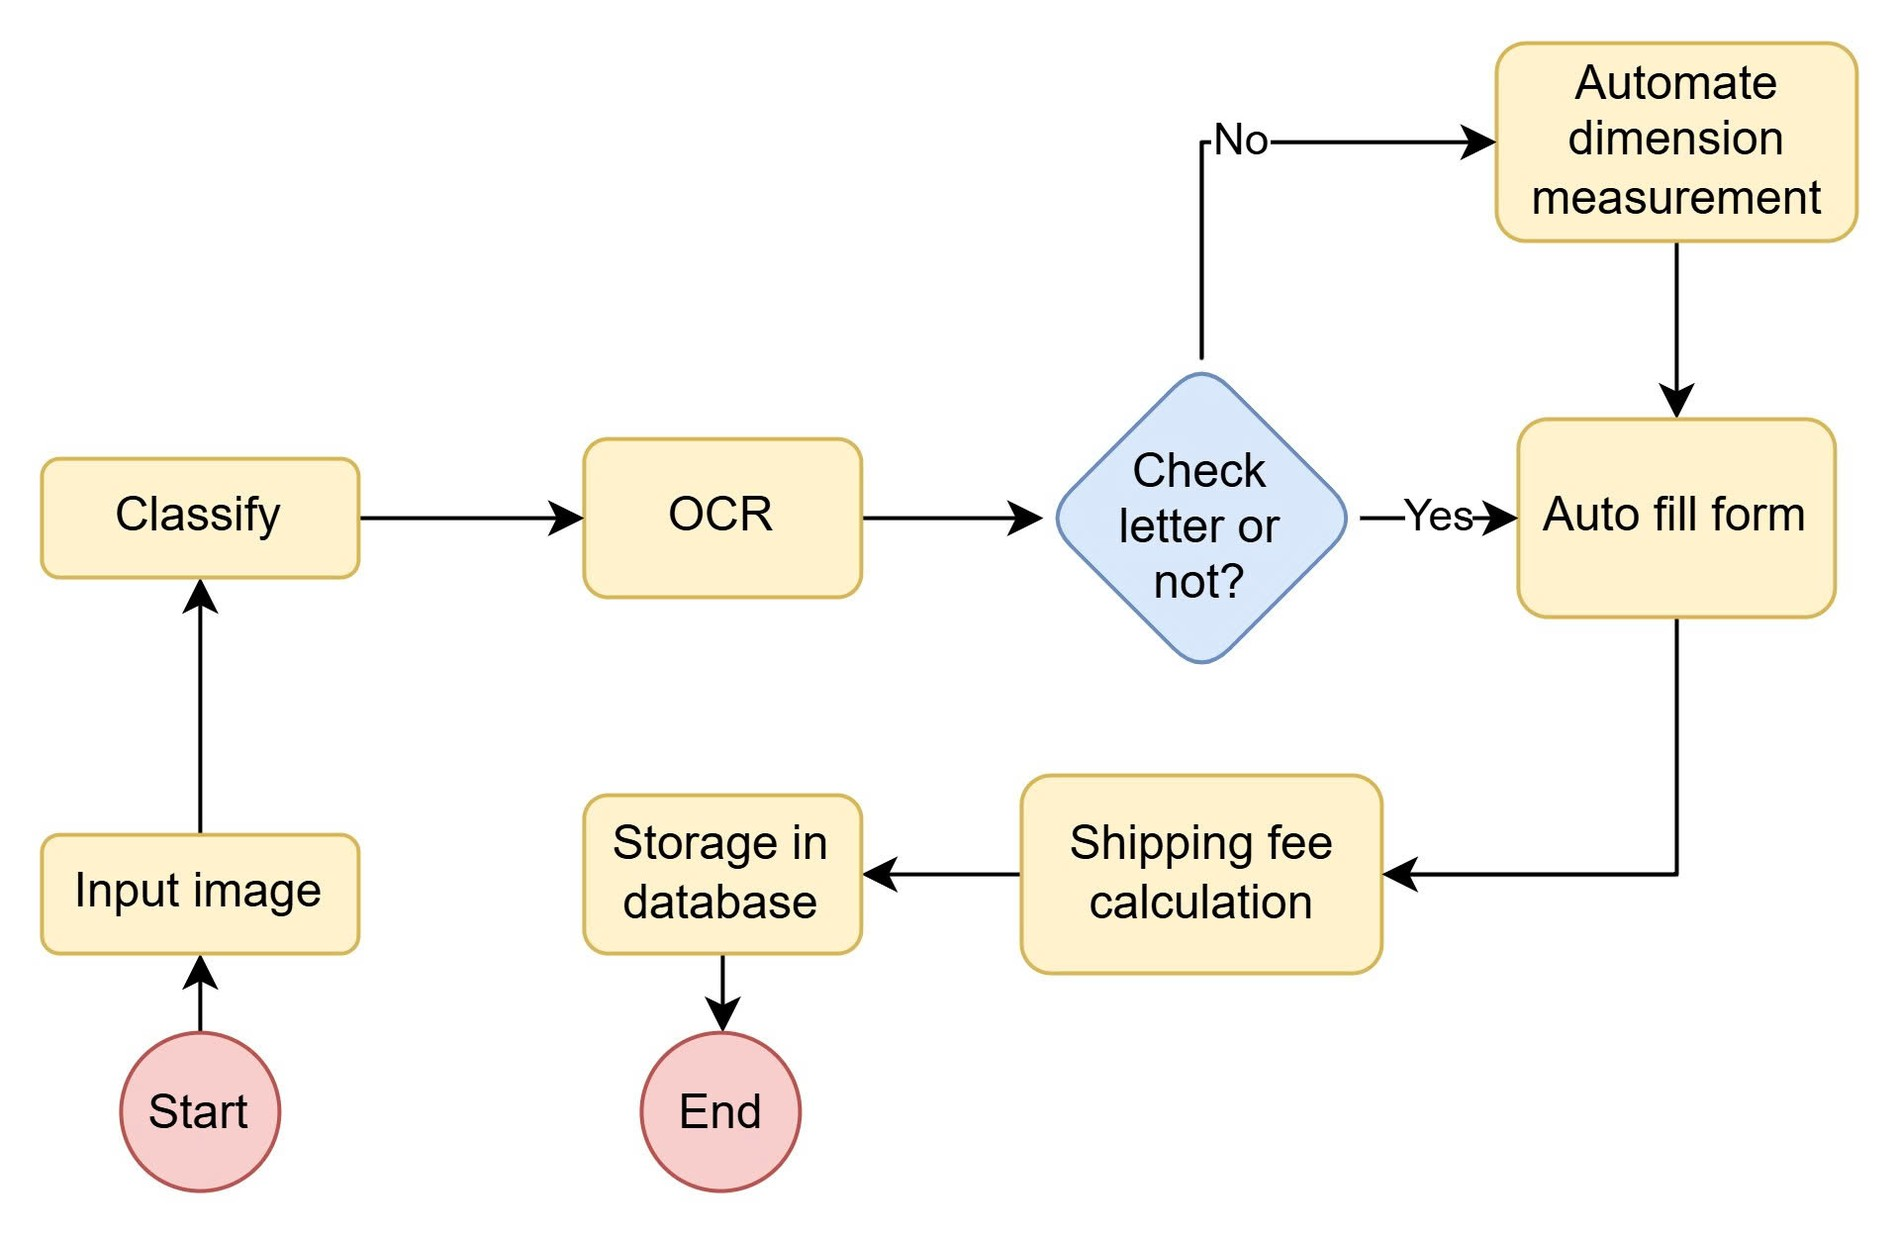
\includegraphics[width=\textwidth]{Images/fig4_2.jpg}
\caption{Overall processing workflow of the proposed system.}
\label{fig:workflow}
\end{figure}

First, the system receives the postal item image and uses the Box/Envelope Detection module to determine whether the input is a parcel or an envelope. The image is then passed through the OCR pipeline to detect and recognize the handwritten information. Both item types use the same OCR pipeline, but the way the input region is prepared differs. For envelopes, the envelope region is cropped and passed directly to the text region detection step. For parcels, the system additionally uses Information Region Detection to locate and crop the information label region before recognizing the handwriting.

The classification result is retained in order to determine the subsequent processing path. If the item is an envelope, the system skips the dimension measurement step and passes the OCR result to the form. If the item is a parcel, the system additionally performs dimension measurement using webcams or ultrasonic sensors before filling in the form.

Once the form has been filled in, the clerk enters the actual weight and selects the service. The system uses the province information, the weight and the dimensions to calculate the shipping fee. Finally, the transaction information and the fee calculation result are saved to the database.

\section{System Architecture}

Based on the workflow presented above, the system components are organized into three functional groups: postal information extraction and recognition, webcam-based dimension measurement, and ultrasonic-sensor-based dimension measurement. This section presents the structure and the connections between the components of each group; their processing procedures are presented in Section~\ref{sec:algorithm_description}.

\subsection{Postal Information Extraction and Recognition}

Figure~\ref{fig:infoarch} presents the combination of the three functions Box/Envelope Detection, Information Region Detection and Handwriting Recognition.

\begin{figure}[htbp]
\centering
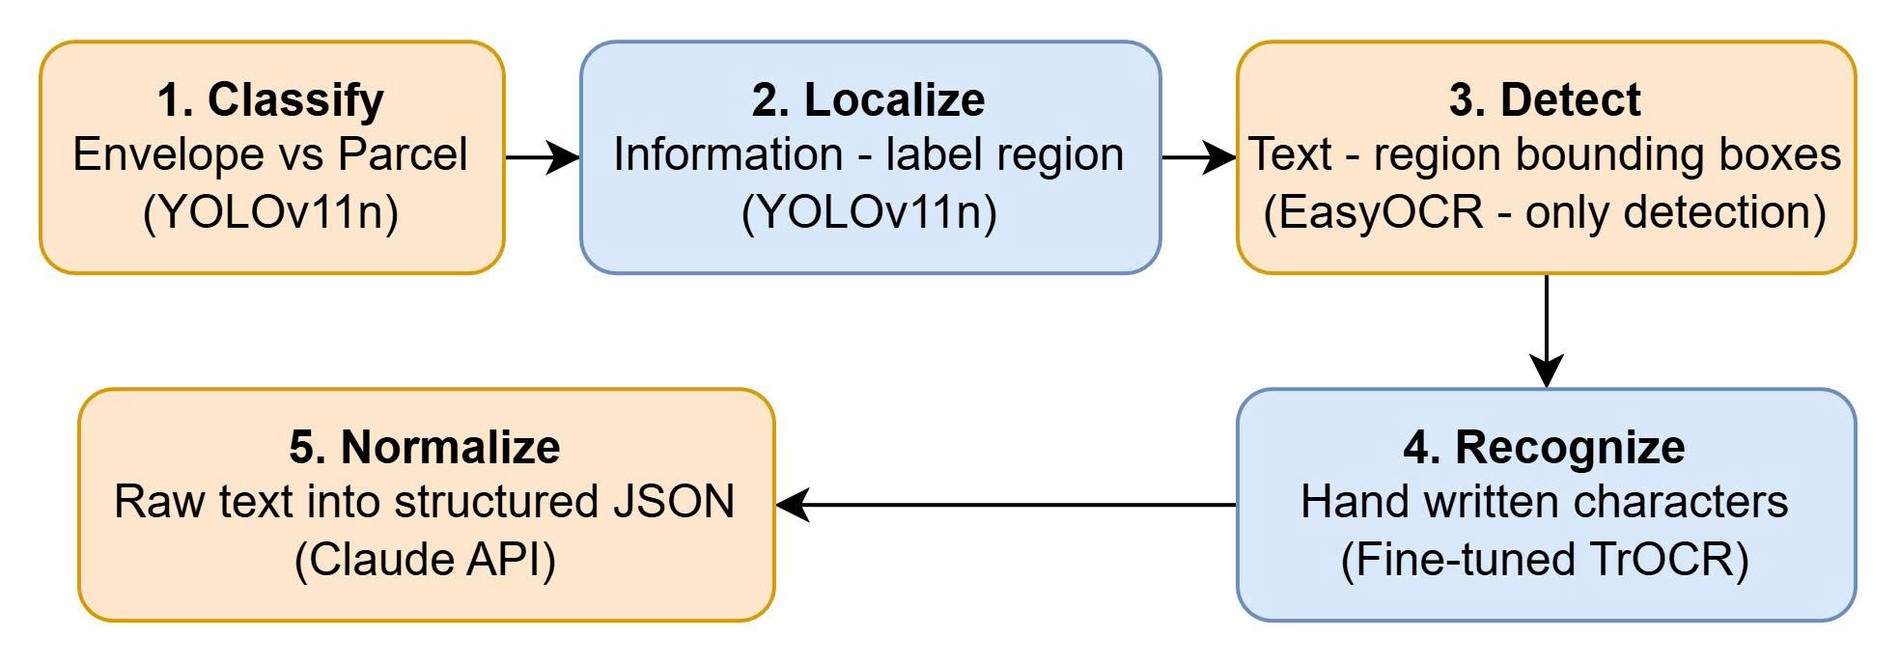
\includegraphics[width=\textwidth]{Images/fig4_3.jpg}
\caption{Architecture of the postal information extraction and recognition module.}
\label{fig:infoarch}
\end{figure}

First, YOLO11n determines whether the item is a parcel or an envelope. This result decides how the image region to be processed is identified. For parcels, a second YOLO11n model locates the information label region on the parcel surface; for envelopes, the envelope image region is used directly. Once the information region has been identified, EasyOCR detects the regions containing text and returns their bounding boxes. Each text region is then passed to the fine-tuned TrOCR model to recognize the handwritten content. Finally, the recognized text is reordered and converted into structured JSON data through the Claude API.

\subsection{Webcam-Based Dimension Measurement}

The architecture of the webcam-based measurement system is shown in Figure~\ref{fig:webcamarch}. It consists of four main components.

\begin{figure}[htbp]
\centering
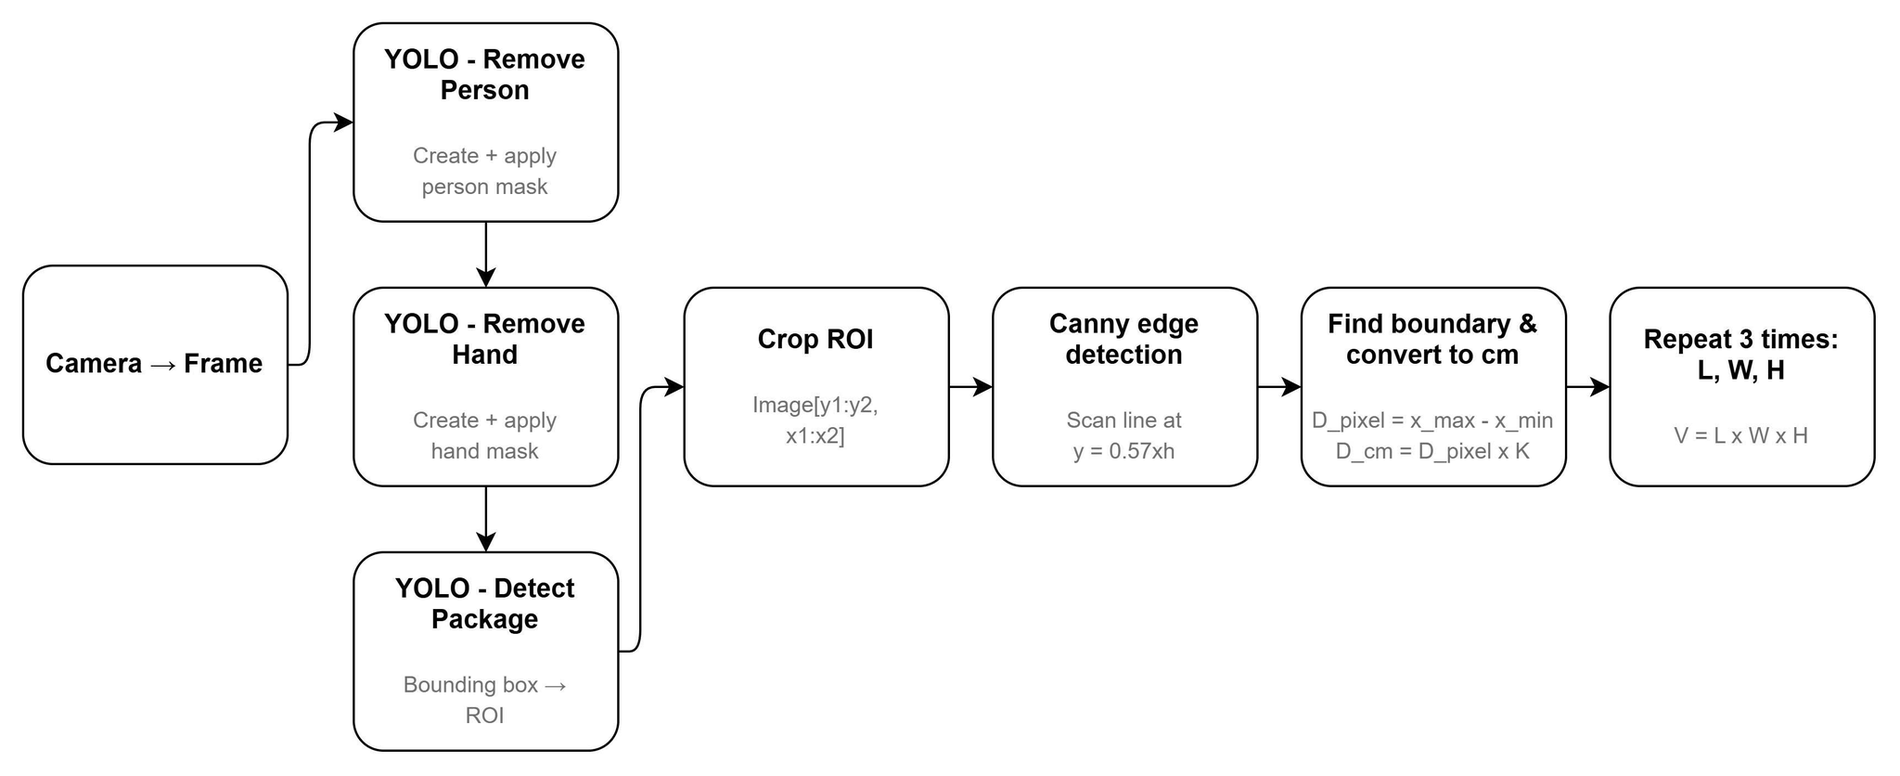
\includegraphics[width=\textwidth]{Images/fig4_4.png}
\caption{Architecture of the two-webcam dimension measurement system.}
\label{fig:webcamarch}
\end{figure}

\begin{itemize}
    \item \textbf{YOLO26n Person Detection:} detects human body regions that may appear in the image.
    \item \textbf{YOLO Hand Keypoints:} detects hands and their keypoints in order to identify the regions to be removed.
    \item \textbf{YOLO Package Detection:} determines the bounding box of the parcel and creates the region of interest.
    \item \textbf{Dimension Measurement:} detects edges within the region of interest, determines the dimensions in pixels and converts them into centimetres.
\end{itemize}

The person and hand regions are masked before parcel boundary detection. This step limits cases in which the body or hand is mistaken for part of the parcel boundary. The bounding box returned by YOLO Package Detection is used to crop the region of interest, after which Canny edge detection identifies the edges used for measurement \cite{canny1986}.

\subsection{Ultrasonic-Sensor-Based Dimension Measurement}

The architecture of the ultrasonic measurement system is shown in Figure~\ref{fig:ultrasonicarch}. It consists of three main blocks.

\begin{figure}[htbp]
\centering
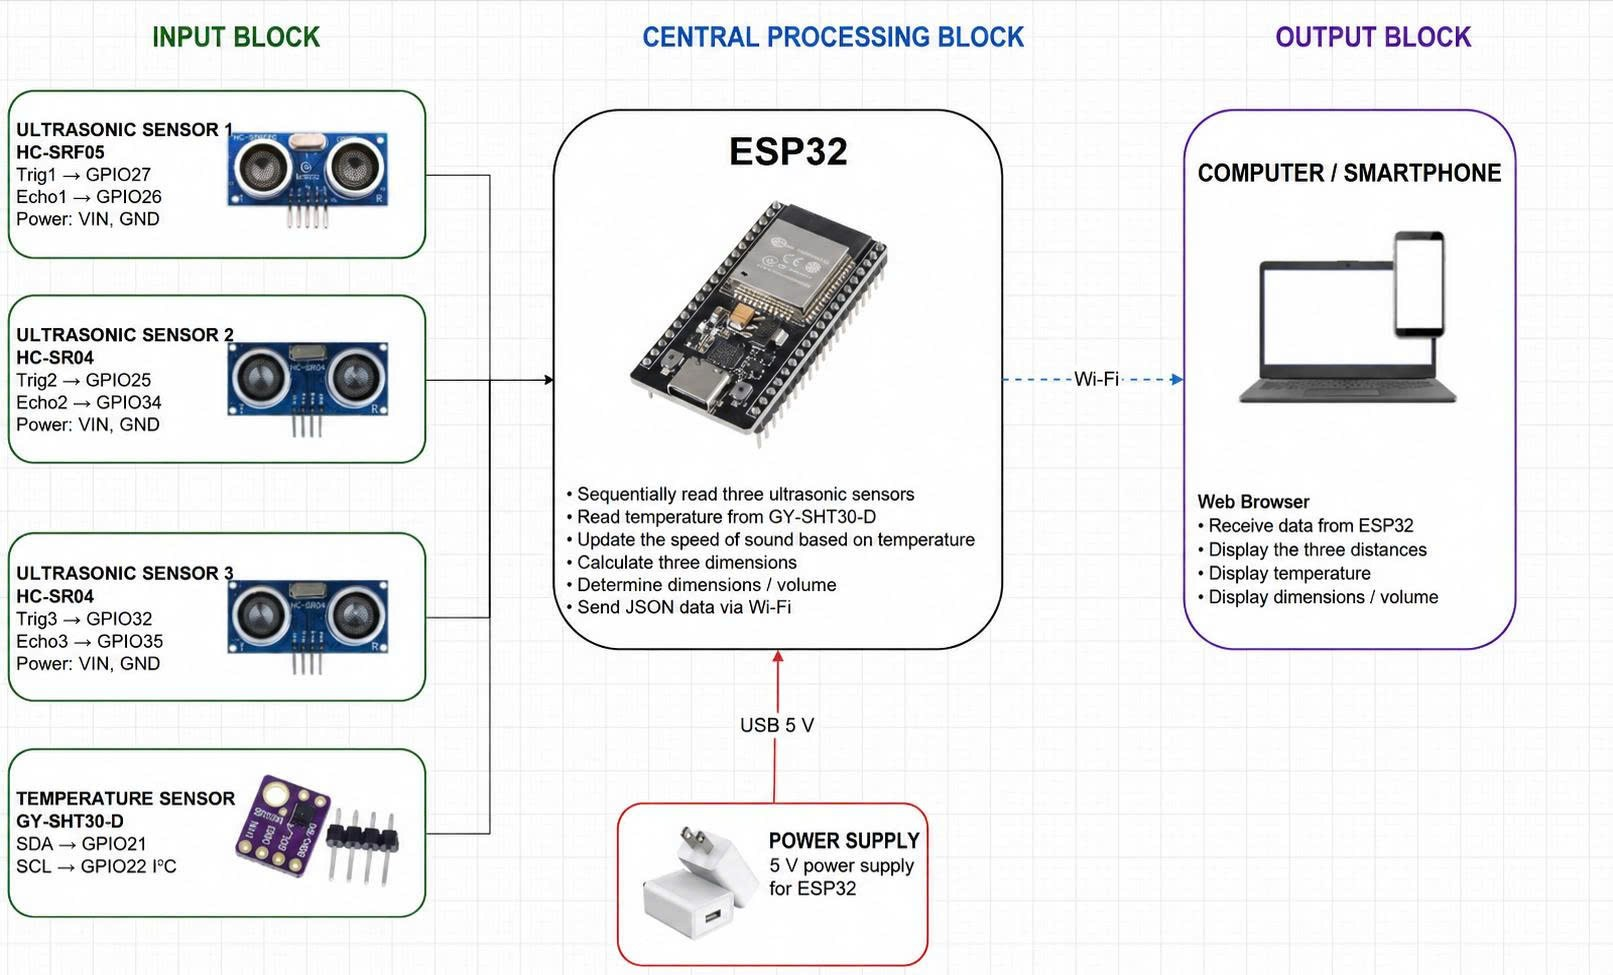
\includegraphics[width=\textwidth]{Images/fig4_5.jpg}
\caption{Architecture of the ultrasonic-sensor dimension measurement system.}
\label{fig:ultrasonicarch}
\end{figure}

The input block contains three ultrasonic sensors for distance measurement and an \mbox{SHT30-D} sensor for ambient temperature measurement. The sensor data is transmitted to the ESP32 in the central processing block. The ESP32 reads the three ultrasonic sensors in turn, updates the speed of sound according to the temperature, determines the three distances and computes the length, width, height and volume of the parcel. The result is packaged as JSON and sent over Wi-Fi. The output block is a browser on a computer or phone; the interface receives the data from the ESP32 and displays the temperature, the three distances, and the dimensions and volume of the parcel.

\section{Algorithm Description}
\label{sec:algorithm_description}

\subsection{Box/Envelope Detection}

The study uses YOLO11n to detect and distinguish parcels from envelopes. Rather than training from scratch, the model is initialized from the pretrained weights \texttt{yolo11n.pt} and then fine-tuned on the Postal Item Dataset. The model uses two classes, \texttt{Label\_Box} and \texttt{Label\_Envelope}; the \texttt{Label\_info} class is not used when training this model because it is not needed for distinguishing the two item types.

\begin{figure}[htbp]
\centering
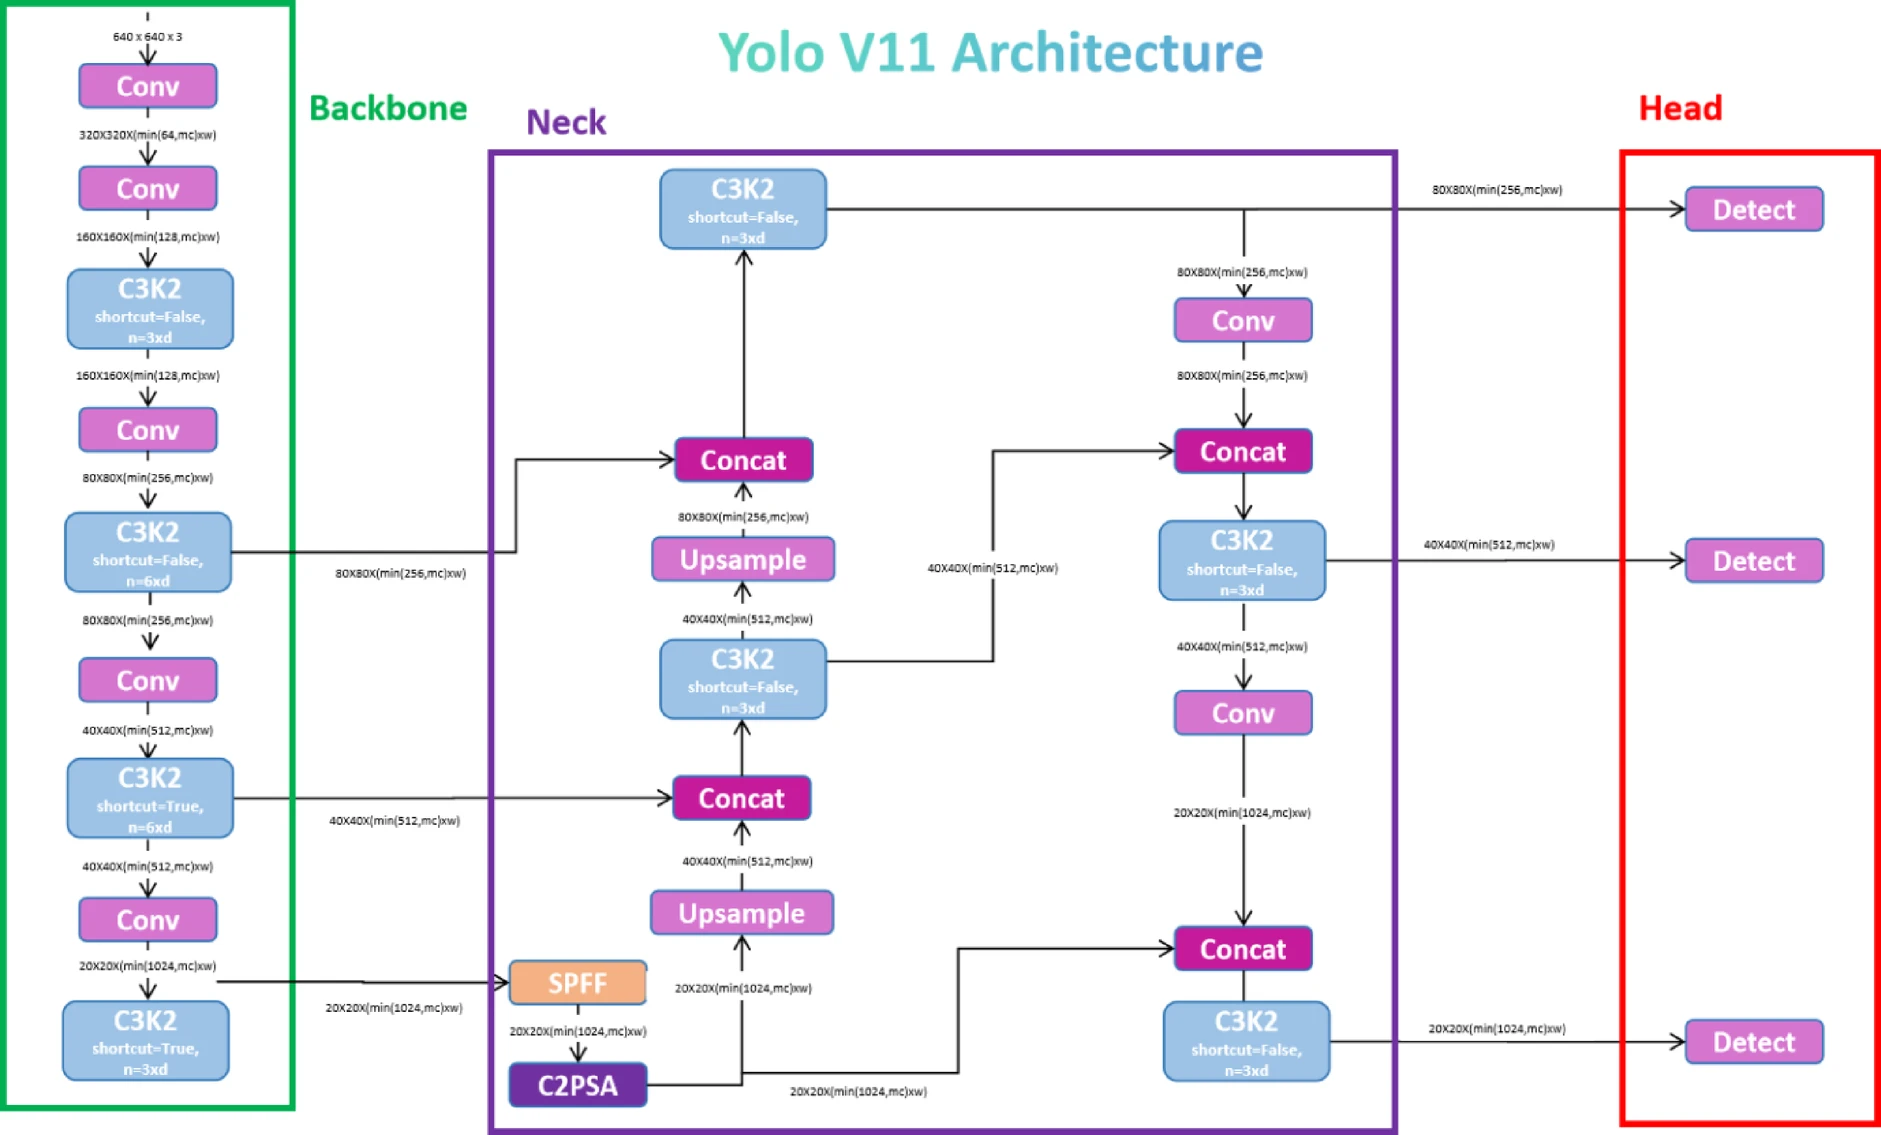
\includegraphics[width=\textwidth]{Images/fig4_6.png}
\caption{General architecture of YOLO11n.}
\label{fig:yolo11n}
\end{figure}

As shown in Figure~\ref{fig:yolo11n}, YOLO11n is a single-stage object detection model whose operation consists of three main steps: feature extraction, object prediction and result post-processing. At a high level, the architecture has three components \cite{ultralytics_yolo11}:

\begin{itemize}
    \item \textbf{Backbone:} extracts features from the input image. The early layers learn basic features such as edges, shapes and textures, while the deeper layers produce features with a higher semantic level.
    \item \textbf{Neck:} combines the extracted features across multiple levels and scales.
    \item \textbf{Detection head:} uses the combined features to predict bounding boxes, class labels and confidence scores.
\end{itemize}

The model output consists of a bounding box giving the position and size of the object, a class indicating whether the object is a \texttt{Label\_Box} or a \texttt{Label\_Envelope}, and a confidence score. The overlap between the predicted bounding box and the ground-truth bounding box is measured by the intersection over union, defined in Equation~\eqref{eq:iou}:

\begin{equation}
\label{eq:iou}
\mathrm{IoU} = \frac{\mathrm{Area}\left(B_{\mathrm{pred}} \cap B_{\mathrm{gt}}\right)}{\mathrm{Area}\left(B_{\mathrm{pred}} \cup B_{\mathrm{gt}}\right)}
\end{equation}

where $B_{\mathrm{pred}}$ is the bounding box predicted by the model and $B_{\mathrm{gt}}$ is the annotated ground-truth bounding box. A larger value indicates a greater overlap between the two bounding boxes. After the model produces its predictions, a confidence threshold is used to discard low-confidence results, and non-maximum suppression removes duplicate bounding boxes when several predictions identify the same object \cite{ultralytics_yolo11}. The final result provides the postal item type and the position of the object in the image, which is passed to the next processing step.

\subsection{Information Region Detection}

Information Region Detection uses a second YOLO11n model and is only performed when the item has been identified as a box. The parcel region is cropped from the original image using the bounding box from Box/Envelope Detection, and the cropped image is fed into Information Region Detection to locate the area containing the information label. This model uses only one class, \texttt{Label\_info}.

Once the bounding box of the information region has been determined, this area is cropped to remove the irrelevant parts of the parcel surface, and the information region image is passed to the handwriting recognition pipeline. For envelopes, Information Region Detection is not used: the envelope region is cropped from the Box/Envelope Detection result and passed directly to the text region detection step.

\subsection{Handwriting Recognition}

The handwriting recognition system has two stages. The first is fine-tuning TrOCR on Vietnamese handwriting data; the second is using the trained model to recognize and extract information from postal item images. The inference pipeline is summarized below.

\begin{center}
\begin{minipage}{\textwidth}
\hrule\vspace{3pt}
\noindent\textbf{Handwritten information extraction pipeline}
\vspace{3pt}\hrule\vspace{4pt}
\begin{algorithmic}[1]
\State \textbf{Input:} RGB image $I$ of the information region
\State $\mathcal{B} \gets \textsc{EasyOCR}(I)$ \Comment{detect text regions with confidence scores}
\State $\mathcal{B} \gets \{b \in \mathcal{B} \mid \mathrm{conf}(b) > 0.4\}$ \Comment{discard low-confidence regions}
\For{each region $b \in \mathcal{B}$}
    \State $t_b \gets \textsc{TrOCR}(I[b])$ \Comment{recognize the handwritten content}
\EndFor
\State $\mathcal{T} \gets \textsc{Split}(\mathcal{B})$ \Comment{identify columns and sender/receiver areas}
\State $\mathcal{T} \gets \textsc{Merge}(\mathcal{T})$ \Comment{join fragments on the same row}
\State $\mathcal{T} \gets \textsc{Pair}(\mathcal{T})$ \Comment{pair label blocks with value blocks}
\State $R \gets$ concatenate the cells of each row, then join the rows
\State \textbf{return} $\textsc{ClaudeAPI}(R)$ \Comment{structured JSON with 11 fields}
\end{algorithmic}
\vspace{2pt}\hrule
\end{minipage}
\end{center}

\textbf{Text region detection.} The input is an RGB image of the information region. CRAFT, via EasyOCR, detects the regions containing text and returns bounding boxes together with confidence scores \cite{baek2019craft, easyocr}. The system keeps only regions with a confidence score greater than 0.4 in order to reduce noise.

\textbf{Handwritten text recognition.} The \texttt{trocr-vietnamese-final} model recognizes the content of each region detected by EasyOCR. The result for each region consists of a text segment and the corresponding bounding box.

\textbf{Layout reconstruction.} The text regions returned by EasyOCR and TrOCR are still fragmented and must be reordered according to the layout of the shipping form. The SPLIT step identifies the columns and the sender and receiver information areas; the MERGE step joins text fragments that lie on the same row, based on their vertical overlap; and the PAIR step pairs a label block with the value block on the same row. Figure~\ref{fig:easyocrregions} shows the text regions produced by EasyOCR, and Table~\ref{tab:layoutexample} illustrates the processing of one row of data. These three steps are a processing method designed by the team for the layout of the shipping form.

\begin{figure}[htbp]
\centering
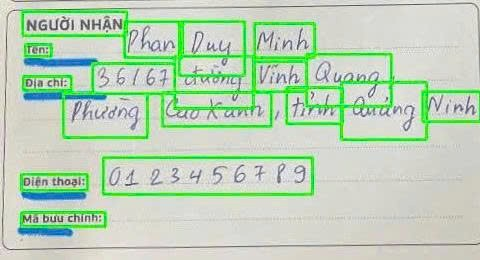
\includegraphics[width=\textwidth]{Images/fig4_7.jpg}
\caption{Text regions detected with EasyOCR.}
\label{fig:easyocrregions}
\end{figure}

\begin{table}[htbp]
\centering
\caption{Example of the layout reconstruction process}
\label{tab:layoutexample}
\small
\begin{tabular}{ll}
\hline
\textbf{Stage} & \textbf{Content} \\
\hline
Fragmented text regions & ``Tên''; ``Phan''; ``Duy''; ``Minh'' \\
After MERGE & ``Tên''; ``Phan Duy Minh'' \\
After PAIR & Label ``Tên'' paired with value ``Phan Duy Minh'' \\
\hline
\end{tabular}
\end{table}

\textbf{Raw text assembly.} Once the logical table has been built, the cells of each row are joined in the correct column order to form a line of text, and the lines are then concatenated with newline characters to produce the complete raw text for each area. For example, if a row has the label ``Họ và tên'' and the value ``John Doe'', the corresponding line of raw text is ``Họ và tên John Doe''.

\textbf{Field extraction.} The raw text is passed to the Claude Sonnet 5 model, \texttt{claude-sonnet-5}, through the Claude API \cite{anthropic_sonnet5}, together with a prompt requesting the extraction of 11 fields: \texttt{sender\_\allowbreak name}, \texttt{sender\_\allowbreak phone}, \texttt{sender\_\allowbreak province}, \texttt{sender\_\allowbreak ward}, \texttt{sender\_\allowbreak address}, \texttt{receiver\_\allowbreak name}, \texttt{receiver\_\allowbreak phone}, \texttt{receiver\_\allowbreak province}, \texttt{receiver\_\allowbreak ward}, \texttt{receiver\_\allowbreak address} and \texttt{item\_\allowbreak description}. The result is returned in JSON format; fields that are not found are set to \texttt{null} and listed in \texttt{missing\_fields} so that the system can request them manually.

\subsection{Webcam-Based Dimension Measurement}

The webcam-based method proceeds as follows. YOLO26n detects the person region and YOLO Hand Keypoints detects hands and their keypoints; both regions are masked. YOLO Package Detection then determines the bounding box of the parcel, which is used to crop the region of interest. Canny edge detection identifies the boundaries within that region, the pixel dimensions are converted into centimetres, and the three dimensions are used to compute the volume.

The first camera is fixed in front of the parcel to determine its horizontal width and height. Because the distance between the camera and the measurement area does not change, each pixel is converted into a real length through a coefficient $K$, as given in Equation~\eqref{eq:pixel2cm}:

\begin{equation}
\label{eq:pixel2cm}
L = p_L \times K, \qquad H = p_H \times K
\end{equation}

where $p_L$ and $p_H$ are the numbers of pixels along the horizontal and vertical directions in the front camera image, $K$ is the conversion coefficient in centimetres per pixel, and $L$ and $H$ are the real horizontal width and height.

The second camera is placed above the parcel and observes both the horizontal width and the depth. Since the real width $L$ has already been determined from the first camera, the depth is derived from the ratio between the two dimensions in the top camera image, as given in Equation~\eqref{eq:depthratio}:

\begin{equation}
\label{eq:depthratio}
W = L \times \frac{p_W}{p'_L}
\end{equation}

where $p_W$ is the number of pixels along the depth direction, $p'_L$ is the number of pixels along the horizontal direction in the top camera image, and $W$ is the real depth of the parcel. Once the three dimensions have been determined, the volume is computed with Equation~\eqref{eq:volume} and sent to the web interface for price calculation.

\subsection{Ultrasonic-Sensor-Based Dimension Measurement}

The measurement algorithm is shown in Figure~\ref{fig:ultrasonicalgo}. First, the ESP32 reads the temperature from the \mbox{SHT30-D} sensor and computes the speed of sound with Equation~\eqref{eq:speedofsound}. The ESP32 then sends a 10-microsecond HIGH pulse in turn to the trigger pin of each ultrasonic sensor. Sequential triggering is used to limit cross-talk between the three sensors.

\begin{figure}[htbp]
\centering
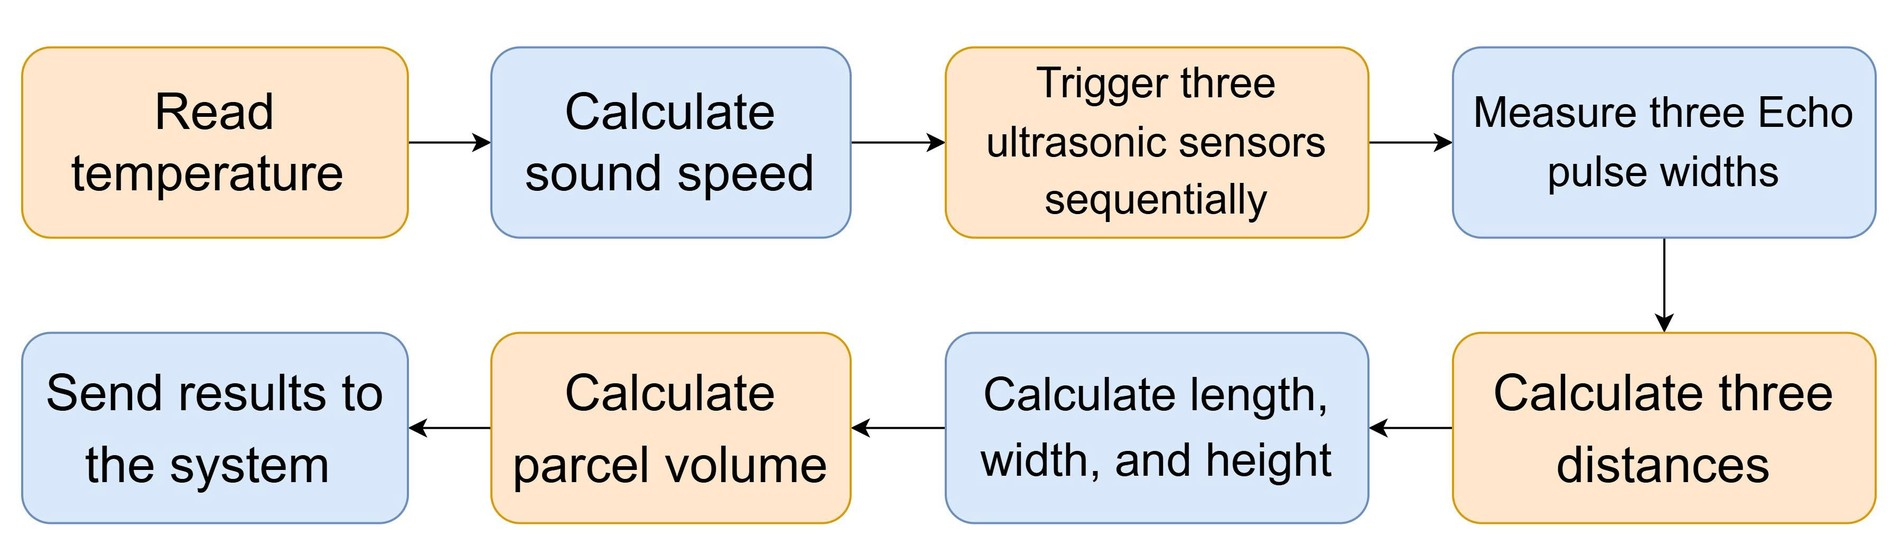
\includegraphics[width=\textwidth]{Images/fig4_8.jpg}
\caption{Algorithm for dimension and volume measurement with ultrasonic sensors.}
\label{fig:ultrasonicalgo}
\end{figure}

Once triggered, each sensor emits a 40\,kHz ultrasonic wave \cite{hcsr04, srf05} towards the parcel and receives the wave reflected from its surface. The ESP32 measures the width of the echo pulse to determine the round-trip travel time, and then computes the distance with Equation~\eqref{eq:tof} \cite{openstax_sound, hcsr04, srf05}. From the three distances obtained, the system determines the parcel dimensions with Equations~\eqref{eq:usL} to \eqref{eq:usH}:

\begin{align}
L &= 105 - d_1 \label{eq:usL}\\
W &= 105 - d_2 \label{eq:usW}\\
H &= 105 - d_3 \label{eq:usH}
\end{align}

\indent where $d_1$, $d_2$ and $d_3$ are the distances from the three sensors to the parcel surface, and $L$, $W$ and $H$ are respectively the length, width and height of the parcel in centimetres. The parcel volume is computed with Equation~\eqref{eq:volume} and sent to the web interface for price calculation.

\subsection{Shipping Fee Calculation}

The fee calculation pipeline, shown in Figure~\ref{fig:feepipeline}, takes as input the service, the origin, the destination, the actual weight and the parcel dimensions. The service codes, route groups, weight tiers and unit prices used in the module were built from the business knowledge base and the 2026 tariff table provided by the post office \cite{vnpost_kb2026, vnpost_tariff2026} (see Appendices~A and~B).

\begin{figure}[htbp]
\centering
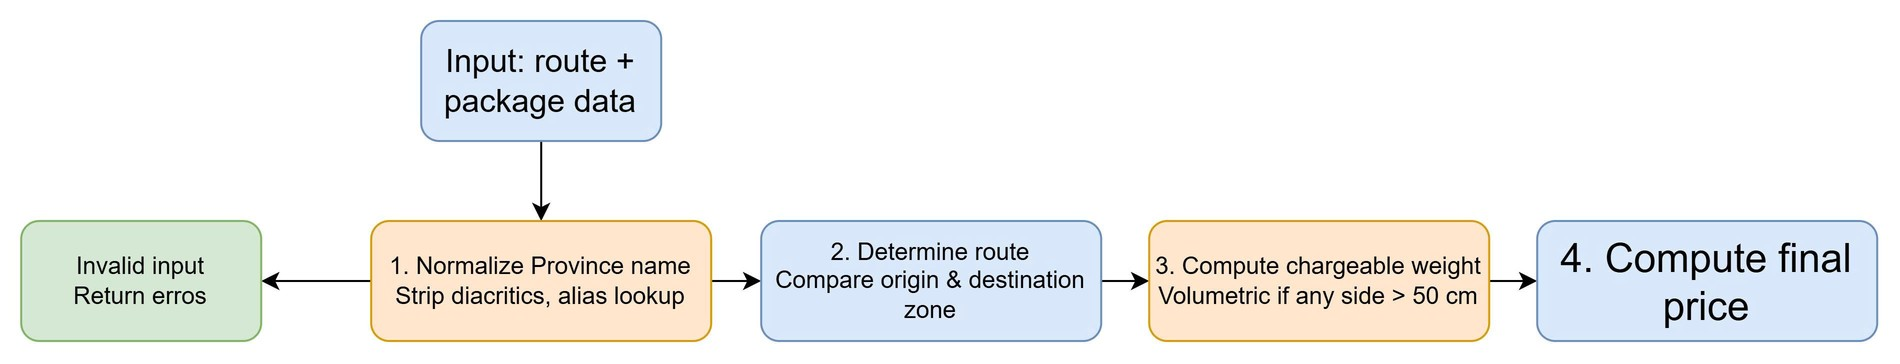
\includegraphics[width=\textwidth]{Images/fig4_9.jpg}
\caption{Shipping fee calculation pipeline.}
\label{fig:feepipeline}
\end{figure}

The calculation consists of four steps.

\textbf{Step 1: province normalization.} The key \texttt{key(province\_input)} is computed by stripping diacritics, lowercasing, and keeping only letters and digits. The alias table is looked up first; if there is no match, the province table \texttt{\_province\_map} is looked up directly; if there is still no match, an invalid-province error is raised. For example, ``Hà nội'' maps to the key \texttt{hanoi} and then to ``Hà Nội'', while ``TP HCM'' maps to \texttt{tphochiminh} and then to ``TP. Hồ Chí Minh''.

\textbf{Step 2: route determination.} The origin and destination are normalized to their canonical names and the zone of each is looked up. If the origin equals the destination the route is intra-province; if both lie in the same zone the route is intra-zone. If the zones differ, then for the ETN service group, covering ETN001, ETN011 and ETN013, the Hà Nội--TP.HCM pair and routes involving Đà Nẵng are assigned to special routes while the rest are inter-zone; for the CTN001 service, the route is near-zone if either end lies in Zone 3 and far-zone otherwise. This division is configured according to the corresponding business documentation and tariff table structure \cite{vnpost_kb2026, vnpost_tariff2026} (see Appendices~A and~B).

\textbf{Step 3: chargeable weight computation.} The volumetric weight is computed as \texttt{weight\_volumetric} $= (L \times W \times H)/6000$. According to the business guidance provided by post office staff, within the scope of this experimental module the volumetric weight is considered when at least one edge of the parcel exceeds 50\,cm; in that case the chargeable weight is the larger of the actual weight and the volumetric weight \cite{vnpost_kb2026} (see Appendix~A). If no edge exceeds 50\,cm, the system uses the actual weight.

\textbf{Step 4: final price computation.} The \texttt{route\_index} corresponding to the route and service is looked up. For CTN001, \texttt{base\_tiers} gives the base price and the base threshold \texttt{base\_limit}; if the weight exceeds the threshold, the cost of each tier in \texttt{progressive\_tiers} into which the excess weight falls is accumulated. For the ETN group, \texttt{base\_tiers} gives the base price and the threshold; if the threshold is exceeded, a surcharge equal to the number of excess units \texttt{unit\_grams} multiplied by the surcharge unit price of the corresponding route is added. The module returns a result object containing the service, the route, the actual weight, the chargeable weight, a flag indicating whether the volumetric weight was used, and the final amount. The base price, the next weight unit and the unit price of the excess portion for each service are taken from the 2026 tariff table \cite{vnpost_tariff2026} (see Appendix~B).

The main parameters of the module are listed in Table~\ref{tab:feeparams}.

\begin{table}[htbp]
\centering
\caption{Main parameters of the fee calculation module}
\label{tab:feeparams}
\small
\begin{tabular}{R{6.2cm}R{7.0cm}}
\hline
\textbf{Parameter} & \textbf{Value or meaning} \\
\hline
Volumetric conversion factor & 6000, following the industry standard $(L \times W \times H)/6000$ in kilograms \\
Threshold for applying volumetric weight & longest edge greater than 50\,cm \\
Surcharge rounding unit for ETN services & \texttt{unit\_grams}, for example 500\,g \\
Number of supported services & 5: LETTER, ETN001, ETN011, ETN013, CTN001 \\
\hline
\end{tabular}
\end{table}

\section{Hyperparameter and Training Setup}
\label{sec:training}

\subsection{Data Splitting Strategy}

The split applied to each model is shown in Table~\ref{tab:datasplit}.

\begin{table}[htbp]
\centering
\caption{Data splits for the models used in this project}
\label{tab:datasplit}
\small
\begin{tabular}{R{3.6cm}R{3.8cm}rrr}
\hline
\textbf{Model} & \textbf{Dataset} & \textbf{Train} & \textbf{Val.} & \textbf{Test} \\
\hline
Box/Envelope Detection & Postal Item Dataset & 1,050 & 44 & 44 \\
Information Region Detection & Postal Item Dataset & 503 & 22 & 22 \\
TrOCR & Viet-\hspace{0pt}Handwriting-\hspace{0pt}OCR-v2 & 58,247 & 1,000 & 1,000 \\
YOLO Package Detection & Cardboard Box Detection & 7,373 & 922 & 921 \\
YOLO Hand Keypoints & Hand Keypoints Dataset & 18,776 & 3,996 & 3,996 \\
\hline
\end{tabular}
\end{table}

For Box/Envelope Detection, the training set was augmented from 351 to 1,050 images, while the validation and testing sets were kept unchanged at 44 images each. For Information Region Detection, only images containing parcels were selected; after cropping the parcel region and converting the coordinates of the \texttt{Label\_info} class, the dataset consists of 503 training images, 22 validation images and 22 testing images.

Viet-Handwriting-OCR-v2 originally consists of 59,247 training samples and 1,000 testing samples. The team used \texttt{train\_test\_split} with \texttt{test\_size = 1000} and \texttt{seed = 42} to separate 1,000 samples from the training set as a validation set. The remaining 58,247 samples were used for training, and the original testing set was kept unchanged for the final evaluation. The fixed seed makes this split reproducible.

YOLO26n Person Detection uses pretrained weights and was not retrained on the project data, so it does not appear in Table~\ref{tab:datasplit}.

\subsection{YOLO11n Training Configuration}

After preprocessing, a new dataset was generated automatically for fine-tuning a second YOLO11n. Information Region Detection has the single task of locating the information label region within the cropped box image, and was trained with parameters similar to Box/Envelope Detection. The configuration is given in Table~\ref{tab:yolocfg}. After training, the best weights of Information Region Detection were saved in the \texttt{weights/best.pt} directory.

\begin{table}[htbp]
\centering
\caption{Training configuration of the two YOLO11n models}
\label{tab:yolocfg}
\small
\begin{tabular}{lll}
\hline
\textbf{Parameter} & \textbf{Box/Envelope Detection} & \textbf{Information Region Detection} \\
\hline
Model & YOLO11n & YOLO11n \\
Pretrained weights & \texttt{yolo11n.pt} & \texttt{yolo11n.pt} \\
Number of classes & 2 & 1 \\
Classes & \texttt{Label\_Box}, \texttt{Label\_Envelope} & \texttt{Label\_info} \\
Epochs & 50 & 50 \\
Image size & $640 \times 640$ & $640 \times 640$ \\
Batch size & 16 & 16 \\
Device & 0 (GPU 0) & 0 (GPU 0) \\
Workers & 4 & 4 \\
\hline
\end{tabular}
\end{table}

\subsection{TrOCR Training Configuration}

The TrOCR fine-tuning process loads the \texttt{microsoft/trocr-base-handwritten} checkpoint, prepares the data with a custom \texttt{TrOCRDataset}, assigns $-100$ to padding tokens so that these positions do not contribute to the loss, freezes the entire encoder and fine-tunes only the decoder. Training is performed with \texttt{Seq2SeqTrainer}, which evaluates and saves a checkpoint every 1,000 steps. The checkpoint with the lowest \texttt{eval\_loss} is selected, and inference is then run on the test set to compute the character error rate and the word error rate with the \texttt{jiwer} library. The configuration is given in Table~\ref{tab:trocrcfg}.

\begin{table}[htbp]
\centering
\caption{TrOCR fine-tuning configuration}
\label{tab:trocrcfg}
\small
\begin{tabular}{R{6.2cm}R{7.0cm}}
\hline
\textbf{Parameter} & \textbf{Value} \\
\hline
Number of epochs & 3 \\
Batch size per device & 2 \\
Gradient accumulation & 4, giving an effective batch size of 8 \\
Learning rate & $1 \times 10^{-5}$ \\
Warmup ratio & 0.1 \\
Optimizer & AdamW, the \texttt{Seq2SeqTrainer} default \\
Regularization & Gradient checkpointing, fp16 mixed precision \\
Evaluation and save steps & Every 1,000 steps, keeping at most 2 checkpoints \\
Best-model selection criterion & Lowest \texttt{eval\_loss}, using \texttt{load\_best\_model\_at\_end} \\
\hline
\end{tabular}
\end{table}

\subsection{Webcam Model Training Configuration}

The webcam system uses one pretrained person detection model and two models fine-tuned for hand detection and parcel detection, on the splits given in Table~\ref{tab:datasplit}. The hyperparameters were kept identical for the two fine-tuning runs, as listed in Table~\ref{tab:hyperparams}.

\begin{table}[htbp]
\centering
\caption{Training parameters used for the webcam system models}
\label{tab:hyperparams}
\small
\begin{tabular}{R{6.2cm}R{7.0cm}}
\hline
\textbf{Hyperparameter} & \textbf{Value} \\
\hline
Number of epochs & 100 \\
Input image size (\texttt{imgsz}) & $640 \times 640$ \\
Batch size & 16 \\
Training device (\texttt{device}) & GPU 0 \\
Number of data loading workers (\texttt{workers}) & 0 \\
\hline
\end{tabular}
\end{table}

Training was carried out on an NVIDIA GeForce RTX 3050 GPU with 4\,GB of VRAM. An image size of $640 \times 640$ was used to standardize the model input. The batch size was set to 16 to fit within the GPU memory limit, while 100 epochs allowed the model to update its weights over many passes through the data. For the webcam-system models, \texttt{workers = 0} was used as a conservative configuration so that data loading was performed in the main process. This setting was specific to these training runs and does not imply that Windows is incompatible with multiprocessing. The two YOLO11n models reported in Table~\ref{tab:yolocfg} were successfully trained with \texttt{workers = 4} on the same machine. YOLO26n Person Detection uses pretrained weights and was not retrained on the project data, so it does not appear in the training configuration.
